\chapter{Projeto e Implementação}

Tendo em vista todos os pontos observados anteriormente, é levantado o perfil da arquitetura do sistema, como pode ser visto na figura a seguir. O projeto foi segmentado em camadas de acordo com a tecnologia sendo implementada (linhas pretas pontilhadas).

Também foram designados microsserviços principais que distinguiam o caminho crítico que desejamos obter. Cada um desses foi descrito neste capítulo.

\begin{figure}[ht]
  \centering
    \includegraphics[scale=0.7]{arquitetura}
  \caption{Diagrama esquemático da arquitetura (Fonte: autores)}
\end{figure}
\FloatBarrier

\section{Módulo Do Target}

Essa etapa engloba possibilitar a comunicação unidirecional de cada dispositivo nos animais (target). Essa comunicação foi feita através da emissão em broadcast de pacotes utilizando Sub-1GHz, que trabalha a frequência de 868MHz, com o protocolo proprietário da Texas Instruments (TI), chamado EasyLink Proprietary RF.

Além disso, era necessário que o target tivesse um ciclo de sleep, de forma a controlar a taxa de transmissão do sinal, reduzindo a energia consumida por cada dispositivo. Alguns estudos foram feitos para se decidir qual a melhor estratégia de implementação.

\subsection{Comunicação unidirecional}

Para tal, o módulo padrão de transmissão (Tx) disponibilizado pela TI foi estudado e modificado sutilmente para que o pacote enviado contivesse o ID de cada animal - que ficou codificado de maneira pré definida (hardcoded) em cada SensorTag.

Esse módulo cria uma task para a execução da tarefa de emissão dos pacotes cujo payload e endereço de destino podem ser configurados. Como só era desejado o ID do macaco e a intensidade do sinal, o payload foi constituído somente por um único byte contendo a primeira informação. Tendo isso em vista, é compreensível que seria possível inserir no mesmo payload demais informações relativas aos animais através dos sensores em cada placa.

Regular a potência do sinal é interessante uma vez que tanto o alcance do sinal quanto a precisão observada no RSSI variam. Adotamos uma intensidade arbitrária de 12 dB para a qual observamos que para cerca de 30 metros o ponto de acesso ainda recebia resposta.

\subsection{Temporização}

Para controle do ciclo de envio e sleep do módulo target, foram pesquisadas três principais estratégias:

\begin{enumerate}
  \item Utilização de um periférico do microcontrolador do SensorTag do tipo timer, para determinação do período de sleep através de seu contador;
  \item Por meio de uma pausa na tarefa do sistema operacional que está executando a transmissão de pacotes;
  \item Ou alterando-se uma constante da estrutura de pacotes.
\end{enumerate}

A Texas Instruments permite que o controle dos periféricos dos módulos utilizados seja feito por meio do uso de APIs específicas de seus drivers. No caso do timer, é possível utilizar a referência da biblioteca GPTimerCC26XX.h \cite{gptimer}. Ela contém funções básicas de operação do timer, como init(), start(), stop() e callback().

Para utilização do timer, é necessário também que se configure seus parâmetros. Alguns deles, mais essenciais, são:

\begin{itemize}
	\item views de cadastro, edição e listagem;
	\item um controlador, para mapear as requisições REST;
	\item um repositório;
	\item um serviço, para atuar no repositório.
\end{itemize}

Todos esses parâmetros são referenciados no datasheet do microcontrolador \cite{datasheet} e na referência da biblioteca do driver \cite{gptimer}. No contexto do sensortag e deste projeto, o timer pode ser configurado para funcionar de maneira periódica e a transmissão de mensagens ser incluída em sua função de callback.

O cálculo da periodicidade do timer deve ser feita levando-se em conta a sua frequência de atualização, lembrando que, em uma descrição simples, o funcionamento do timer consiste em contar de 0 até o valor especificado em seus parâmetros. O memorial de cálculo encontra-se no Apêndice 4.

Boa parte dos exemplos de uso de periféricos providos pela Texas Instruments incluem criação de tasks. Conforme mencionado no início do capítulo 6, utilizou-se primariamente um dos exemplos fornecidos pela TI para operação do módulo de target. Uma solução mais simples do que configurar o timer (e possivelmente menos custosa) seria utilizar a função Task\texttt{\char`_}Sleep(nticks) \cite{task-modules}. O que esta função faz em essência é bloquear a task pelo tempo definido em nticks, o qual é medido em ms e tem como referência o próprio clock do sistema (48MHz \cite{datasheet}).

Uma última estratégia seria utilizar um dos parâmetros da própria estrutura de mensagens de Tx do protocolo utilizado \cite{forum-easylink}. Tal parâmetro é EasyLink\texttt{\char`_}ms\texttt{\char`_}To\texttt{\char`_}RadioTime e é medido em ms, como seu nome sugere \cite{easylink}. Seria uma alternativa às duas últimas mencionadas, porém, há pouca informação sobre seu tamanho máximo e há relatos de outros usuários da API sobre bugs em seu uso por este motivo.

\subsection{Eficiência Energética}

Para efeito de preservação da bateria foi escolhida uma taxa de transmissão de 5 segundos de maneira a manter o aspecto de atualização em tempo real. Tal valor pode ser configurado facilmente alterando-se uma das variáveis mencionadas nas estratégias de temporização mencionadas anteriormente (loadVal para o timer, nTicks para Task\texttt{\char`_}Sleep() e EasyLink\texttt{\char`_}ms\texttt{\char`_}To\texttt{\char`_}RadioTime para a estrutura dos pacotes). Esta mudança deve ser feita caso seja julgada interessante uma maior economia de energia em troca de desempenho.

\section{Módulo Do Ponto De Acesso}

Cada ponto de acesso é responsável pela leitura e armazenamento dos dados correspondentes aos pacotes enviados pelos targets. Assim, para cada pacote recebido é possível identificar a intensidade do sinal, que é armazenada em um vetor de tamanho fixo junto com o ID do macaco.

Uma vez que o vetor estiver completo, o ponto de acesso cria e envia pacotes de maneira similar a como é feita pelos targets, mas com endereço de destino distinto, por exemplo 0xBB.

Para isso, foi desenvolvido um projeto composto por ambos os módulos padrão de leitura (Rx) e transmissão (Tx). O módulo de leitura é configurado para que passem pelo filtro somente pacotes cujo endereço de destino seja igual ao dos enviados pelo target, por exemplo 0xAA.

\section{Módulo Central}

A mediação da comunicação entre o ponto de acesso (SensorTag) e o controlador (Raspberry Pi) deve ser feita através do nó denominado Central implementado por um SensorTag conectado por UART ao controlador.
Este componente terá a função de receber os pacotes filtrados pelo endereço de destino configurado pelos pontos de acesso e repassar as informações por conexão serial para o controlador.

Para isso, analogamente ao realizado nos demais componentes, foi desenvolvido um projeto composto por ambos os módulos padrão de leitura (Rx) e transmissão serial UART disponibilizados pela TI. Essa composição foi feita criando uma thread para cada módulo utilizando buffers duplos, de forma que cada tarefa trabalhasse paralelamente em um buffer individual.

O tamanho dos buffers foi dimensionado para abrigar 32 medidas, considerando a memória máxima da placa e, ao mesmo tempo, a não sobrecarregar a comunicação serial com o controlador, que depende da interrupção dessa comunicação para escrever no banco. O módulo UART é configurado para atuar a taxa de transmissão de 115200 bps sem paridade.

\section{Módulo Do Controlador}

Ao receber as informações, o controlador deve formatar os dados das distâncias e timestamps de cada medida tomada. Neste momento os valores de RSSI recebidos devem ser convertidos em distâncias em metros através do equacionamento obtido no item 2.4 deste documento e os timestamps são ajustados para o tempo ao qual o controlador está conectado. Além disso, os valores da mensagem são checados para determinar se a mensagem está completa e coerente, ou seja, se não houve perda de dados durante os envios anteriores e é descartada em caso negativo.

Após receber e processar os dados o controlador deve enviá-los para o banco de dados no servidor. Já que não há problemas de armazenamento no controlador ele deve aguardar para enviar as informações para o banco assim que não houver mensagens sendo recebidas na conexão serial, já que seria demasiadamente custoso para o SensorTag guardar e transmitir suas leituras.

A solução escolhida foi o uso da biblioteca MySQLdb em Python, com a qual os dados são inseridos diretamente no banco de dados utilizando SQL queries. Como é boa prática, as mensagens são analisadas antes que de serem enviada para garantir que os dados se encaixam no que foi definido no banco. Caso haja problemas na conexão com o servidor elas são armazenadas no controlador até que ele consiga se reconectar.

O comportamento previamente descrito é esquematizado pela máquina de estados a seguir:

\begin{figure}[ht]
  \centering
    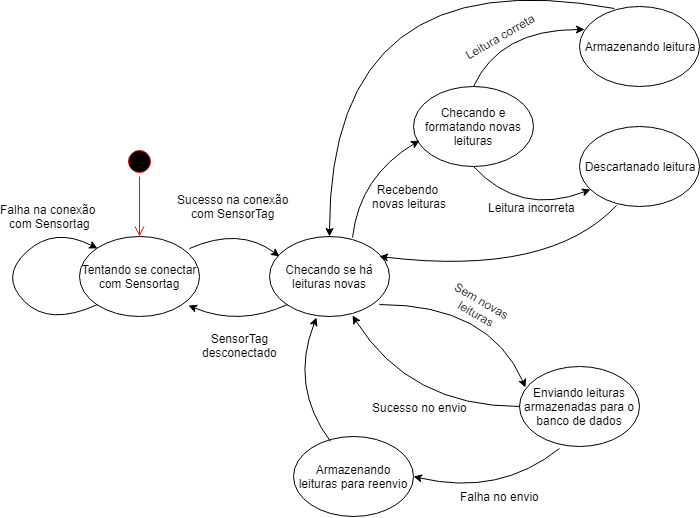
\includegraphics[scale=0.65]{estados-raspberry}
  \caption{Máquina de estados representando o funcionamento do módulo coletor (Fonte: autores)}
\end{figure}
\FloatBarrier

\section{Banco De Dados}

O modelo desenvolvido é relativamente simples e envolve somente os objetos físicos do contexto, de forma que fique claro que são mapeados: o target, o AP e a distância entre eles.

Pelo lado da segurança do sistema, foi utilizado um modelo padrão do Spring Security que mapeia o usuário e suas permissões como pode ser visto no diagrama de classes a seguir.

\begin{figure}[ht]
  \centering
    \includegraphics[scale=0.8]{simios_db}
  \caption{Diagrama de classes gerado pela ferramenta de engenharia reversa do MySQL (Fonte: autores)}
\end{figure}
\FloatBarrier

A implementação do modelo foi feita em código com a declaração das entidades do sistema, que são interpretadas pela API de persistência do Java (JPA). A configuração do banco de dados utilizado (MySQL) ao código permite que o JPA já construa e atualize as tabelas do banco quando necessário.

\section{Banco De Dados}

A interface com o usuário prevê uma aplicação web que permita a visualização dos gráficos e tabelas com dados dos animais.

Para isso, foi utilizado o framework Spring MVC cuja estrutura consistia em considerar a necessidade de implementação de CRUDs para cada um dos objetos principais do sistema que o usuário deve ser capaz de gerenciar: o target, o AP e o usuário. Dessa forma, cada um destes objetos deve possuir:

\begin{itemize}
	\item views de cadastro, edição e listagem;
	\item um controlador, para mapear as requisições REST;
	\item um repositório;
	\item um serviço, para atuar no repositório.
\end{itemize}

A figura a seguir identifica o fluxo de cada uma das telas existentes no sistema. O protótipo das telas é exibido no apêndice 3.

\begin{figure}[ht]
  \centering
    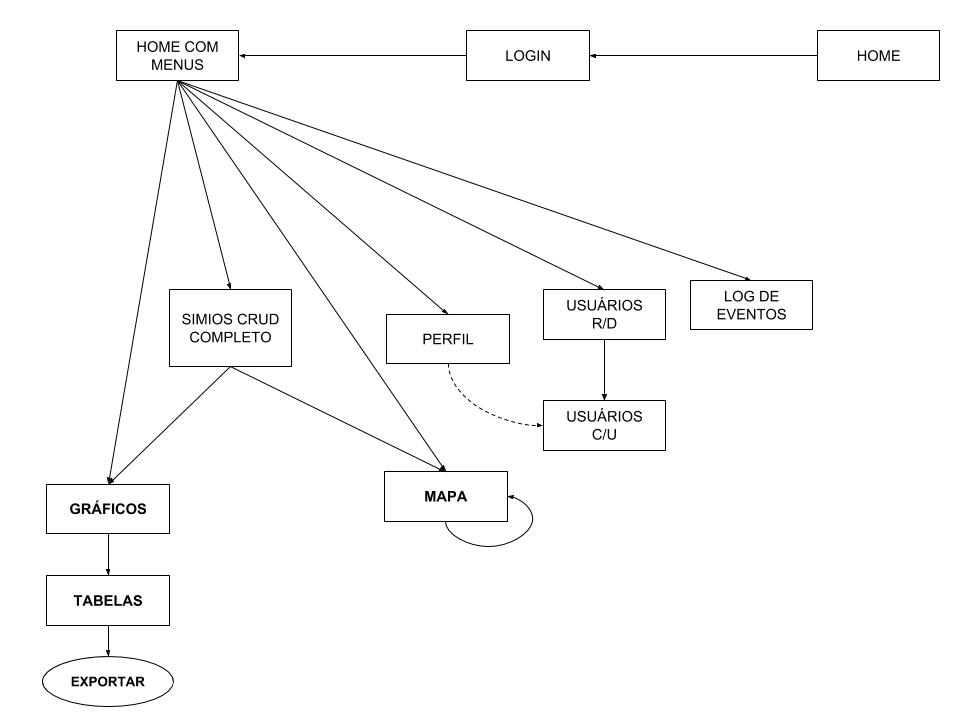
\includegraphics[scale=0.45]{mapa-do-site}
  \caption{Mapa do site (Fonte: autores)}
\end{figure}
\FloatBarrier
